\chapter{pulse width} 
\label{sec:pulse_width}
\lstset{style=6502Style}

\begin{figure}[H]
    \centering
    \begin{adjustbox}{width=10.5cm,margin=0cm}
      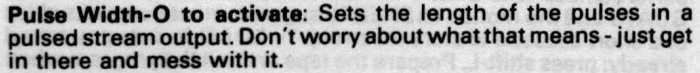
\includegraphics[width=12cm]{src/pulsewidth/pulsewidth.png}%
    \end{adjustbox}
    \caption{
      Excerpt from Manual (Part No. LC1982-Vb). Pulse Width.
      }
\end{figure}

\begin{figure}[H]
    \centering
    \begin{adjustbox}{width=13cm,center}
      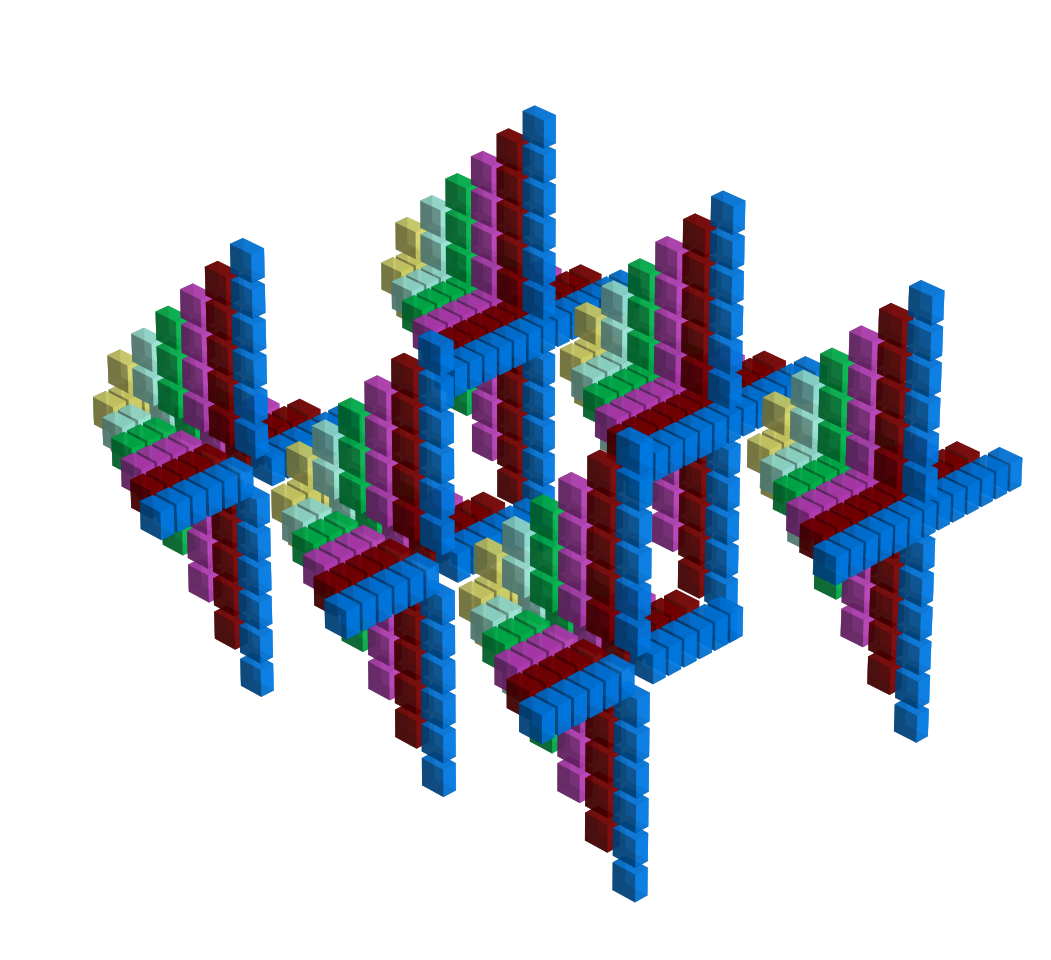
\includegraphics[width=13cm]{src/pulsewidth/pattern0-45.png}%
    \end{adjustbox}
    \caption{Effect of low values for Pulse Width}
\end{figure}
\begin{figure}[H]
    \centering
    \begin{adjustbox}{width=13cm}
      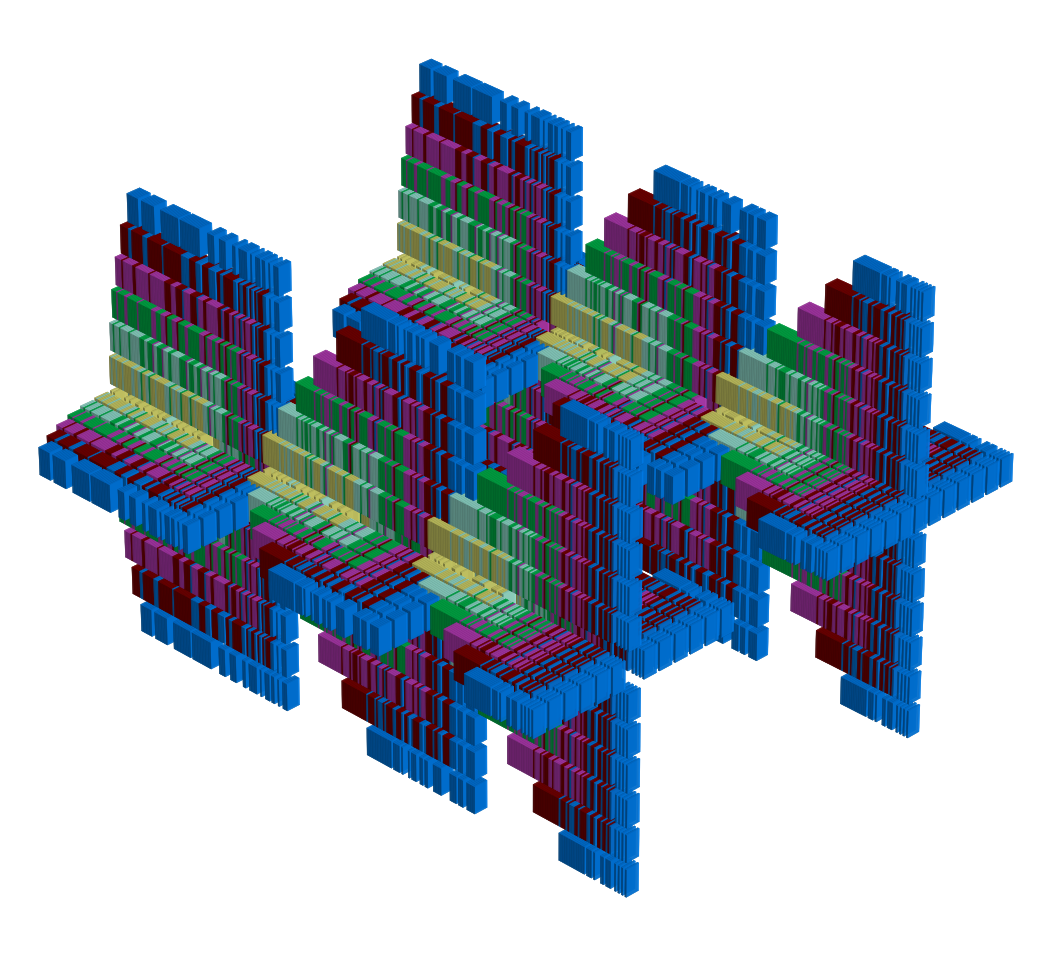
\includegraphics[width=13cm]{src/pulsewidth/pattern1-45.png}%
    \end{adjustbox}
    \caption{Effect of high values for Pulse Width}
\end{figure}


\clearpage
\begin{lstlisting}[caption=From \icode{CheckKeyboardInput}.]
MaybeOPressed   
  CMP #KEY_O ; O pressed.
  BNE MaybeAsteriskPressed

  ; O pressed.
  LDA #PULSE_WIDTH
  STA currentVariableMode
  RTS 
\end{lstlisting}
\begin{lstlisting}[caption=From \icode{CheckKeyboardInputForActiveVariable}. Pressing the < and > keys increments and
decrements the value in presetValueArray pointed to by \icode{X}\, i.e. \icode{currentVariableMode}.]
UpdateVariableDisplay   
  LDA #>SCREEN_RAM + $03D0
  STA colorBarColorRamHiPtr
  LDA #<SCREEN_RAM + $03D0
  STA colorBarColorRamLoPtr

  LDX currentVariableMode
  LDA lastKeyPressed
  CMP #$2C ; > pressed?
  BNE MaybeLeftArrowPressed

  ; > pressed, increase the value bar and write
  ; it to the approiate place in presetValueArray
  INC presetValueArray,X
  LDA presetValueArray,X
  ; Make sure we don't exceed the max value.
  CMP maxValueForPresetValueArray,X
  BNE MaybeInColorMode
  DEC presetValueArray,X
  JMP MaybeInColorMode
\end{lstlisting}

\begin{lstlisting}[basicstyle=\ttfamily\scriptsize,caption=From \icode{ActivateSequencer}.]
; This is where the presets get loaded to. It represents the data structure
; for the presets.currentVariableMode is an index into this data structure
; when the user adjusts settings.
presetValueArray
unusedPresetByte        .BYTE $00
smoothingDelay          .BYTE $0C
cursorWidth             .BYTE $02
bufferLength            .BYTE $1F
pulseWidth              .BYTE $01; <-- Pulse Width is here at position \icode{\$04}.
indexForColorBarDisplay .BYTE $01
lineWidth               .BYTE $07
sequencerWidth          .BYTE $04 
pulseWidth              .BYTE $01
baseLevel               .BYTE $07
presetColorValuesArray  .BYTE BLACK,BLUE,RED,PURPLE,GREEN,CYAN,YELLOW,WHITE
trackingActivated       .BYTE $FF
lineModeActivated       .BYTE $00
presetIndex            .BYTE $05
\end{lstlisting}

\clearpage

\textbf{Lines 1189-1231. \icode{\textbf{DisplayPresetMessage}}:} 
\clearpage


\clearpage
\begin{lstlisting}[caption=From \icode{MainInterruptHandler}.]
DecrementPulseWidthCounter   
        LDA currentPulseWidth
        BEQ DecrementPulseSpeedCounter
        DEC currentPulseWidth
        BEQ DecrementPulseSpeedCounter
        JMP UpdatePixelBuffersForPattern

DecrementPulseSpeedCounter   
        DEC currentPulseSpeedCounter
        BEQ RefreshPulseSpeed
        JMP DrawCursorAndReturnFromInterrupt

RefreshPulseSpeed   
        LDA pulseSpeed
        STA currentPulseSpeedCounter
        LDA pulseWidth
        STA currentPulseWidth

        ; Finally, update the pixel buffers with a byte
        ; each for the current pattern.        
UpdatePixelBuffersForPattern    
        INC currentStepCount
        LDA currentStepCount
        CMP bufferLength
        BNE UpdateBaseLevelArray

        LDA #$00
        STA currentStepCount

\end{lstlisting}
\clearpage

\textbf{Lines 1189-1231. \icode{\textbf{DisplayPresetMessage}}:} 
\clearpage
